%%%%%%%%%%%%%%%%%%%%%%%%%%%%%%%%%%%%%%%%%%%%%%%%%%%%%%%%%%%%%%%%%%%%%%%%
\documentclass[12pt]{article}
\usepackage{amssymb,amsthm}
\usepackage{amsmath,amssymb,CJK}
\usepackage{graphicx}
\usepackage{subfigure}
\usepackage{listings}
\usepackage{enumerate}

\openup 7pt\pagestyle{plain} \topmargin -60pt \textwidth
15cm\textheight 25cm
\parskip .09 truein
\baselineskip 4pt\lineskip 4pt \setcounter{page}{1}
\def\a{\alpha}\def\b{\beta}\def\d{\text{d}}\def\D{\Delta}\def\fs{\footnotesize}
\def\g{\gamma}
\def\G{\Gamma}\def\l{\lambda}\def\L{\Lambda}\def\o{\omiga}\def\p{\psi}
\def\se{\subseteq}\def\seq{\subseteq}\def\Si{\Sigma}\def\si{\sigma}\def\vp{\varphi}\def\es{\varepsilon}
\def\sc{\scriptstyle}\def\ssc{\scriptscriptstyle}\def\dis{\displaystyle}
\def\cl{\centerline}\def\ll{\leftline}\def\rl{\rightline}\def\nl{\newline}
\def\ol{\overline}\def\ul{\underline}\def\wt{\widetilde}\def\wh{\widehat}
\def\rar{\rightarrow}\def\Rar{\Rightarrow}\def\lar{\leftarrow}
\def\Lar{\Leftarrow}\def\Rla{\rightleftarrow}\def\bs{\backslash}
\def\ra{\rangle}\def\la{\langle}\def\hs{\hspace*}\def\rb{\raisebox}
\def\ni{\noindent}\def\hi{\hangindent}\def\ha{\hangafter}
\def\vs{\vspace*}
\def\hom#1{\mbox{\rm Hom($#1,#1$)}}
\def\thebeg{\vskip8pt\par\ni}
\def\theend{\vskip5pt\par}
\def\chabeg{\pagebreak\par}
\def\chaend{\vskip20pt\par}
\def\secbeg{\vskip15pt\par}
\def\secend{\vskip10pt\par}
\def\exebeg{\vskip10pt}
\def\exeend{\vskip6pt}
\def\undot#1{\mbox{$\mbox{#1}\hs{-1.5ex}_{_{\dis\centerdot}}\,\,$}}
\def\qed{\hfill\mbox{$\Box$}}
\def\C{\mathbb{C}}
\def\Q{\mathbb{Q}}
\def\ii{\mbox{\,{\bf i}\,}}
\def\jj{\mbox{\,{\bf j}\,}}
\def\AA{{\cal A}}
\def\BB{{\cal B}}
\def\DD{{\cal D}}
\def\EE{{\mbox{\bf 1}}}
\def\OO{{\mbox{\bf 0}}}
\def\kk{{\mbox{\bf k}}}
\def\R{\mathbb{R}}
\def\F{\mathbb{F}{\ssc\,}}
%\def\similar{\rb{-4pt}{\mbox{\,\~\,}}}
\def\similar{\backsim}
\def\Llra{\Longleftrightarrow}
\def\Lra{\Longrightarrow}
\def\Lla{\Longleftarrow}
\def\mat#1#2{\mbox{$\left(\begin{array}{#1}#2\end{array}\right)$}}
\def\det#1#2{\mbox{$\left|\begin{array}{#1}#2\end{array}\right|$}}
\def\eset{\emptyset}
\parindent=5ex
\setlength{\parindent}{0pt}
\setlength{\parskip}{1ex plus 0.5ex minus 0.2ex}
\def\bf{\mathbf}
\newcommand{\norm}[1]{\left\lVert#1\right\rVert}
\newtheorem{prop}{Proposition}
\date{}
\title{EECS 495 Biometrics Assignment1}
\author{Qinglin Li, EMPL ID: 2923742, Net ID: qlt073\\ Nianzu Li, EMPL ID: 2906237, Net ID: nld118}
\begin{document}
\maketitle
\section*{Problem 1}
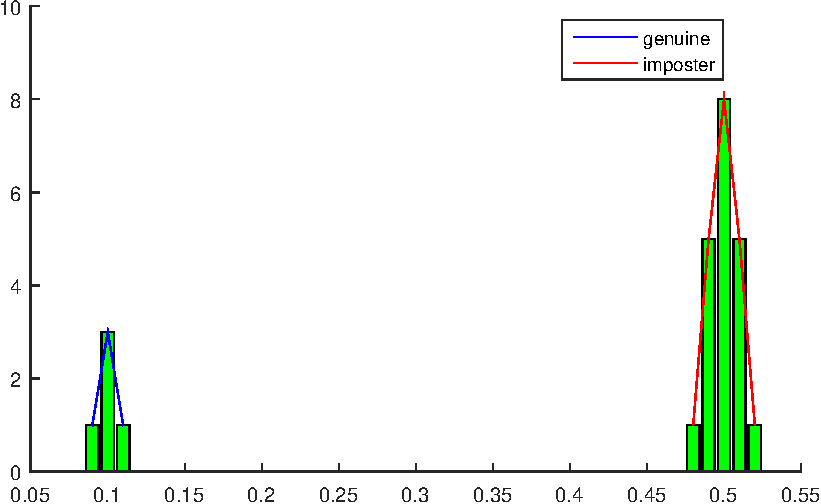
\includegraphics[scale=0.6]{distribution-crop}

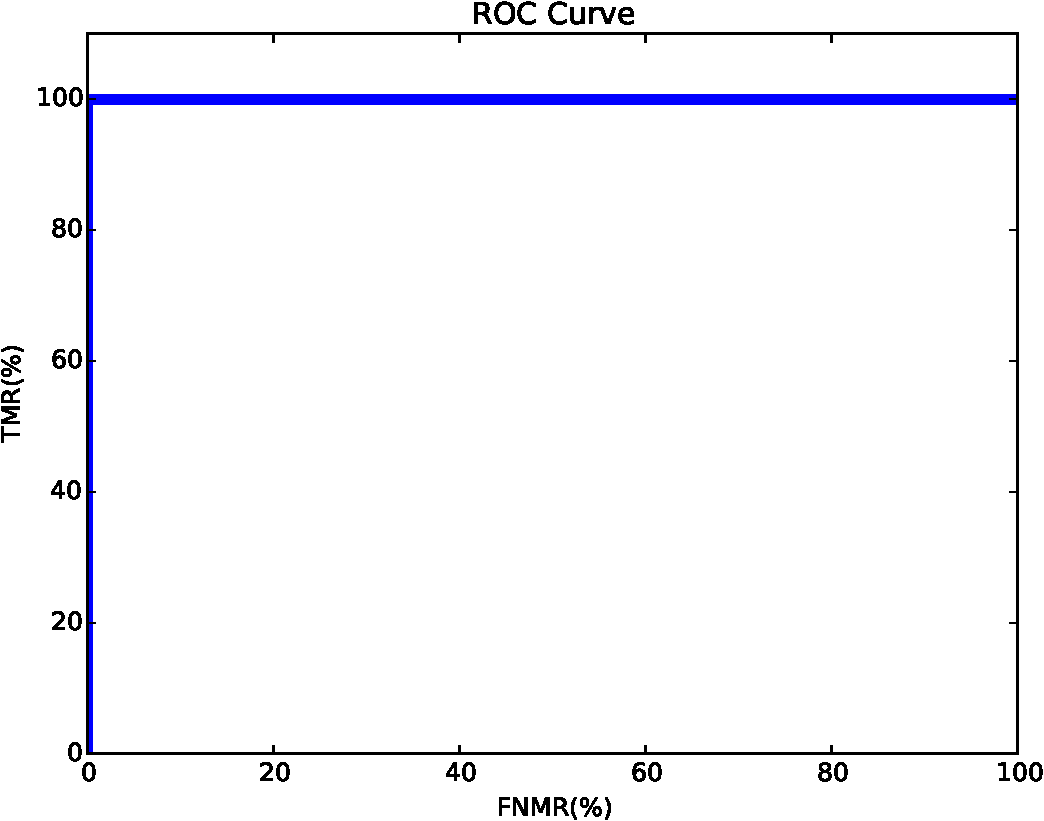
\includegraphics[scale=0.5]{fig-p12-crop}
\section*{Problem 2}
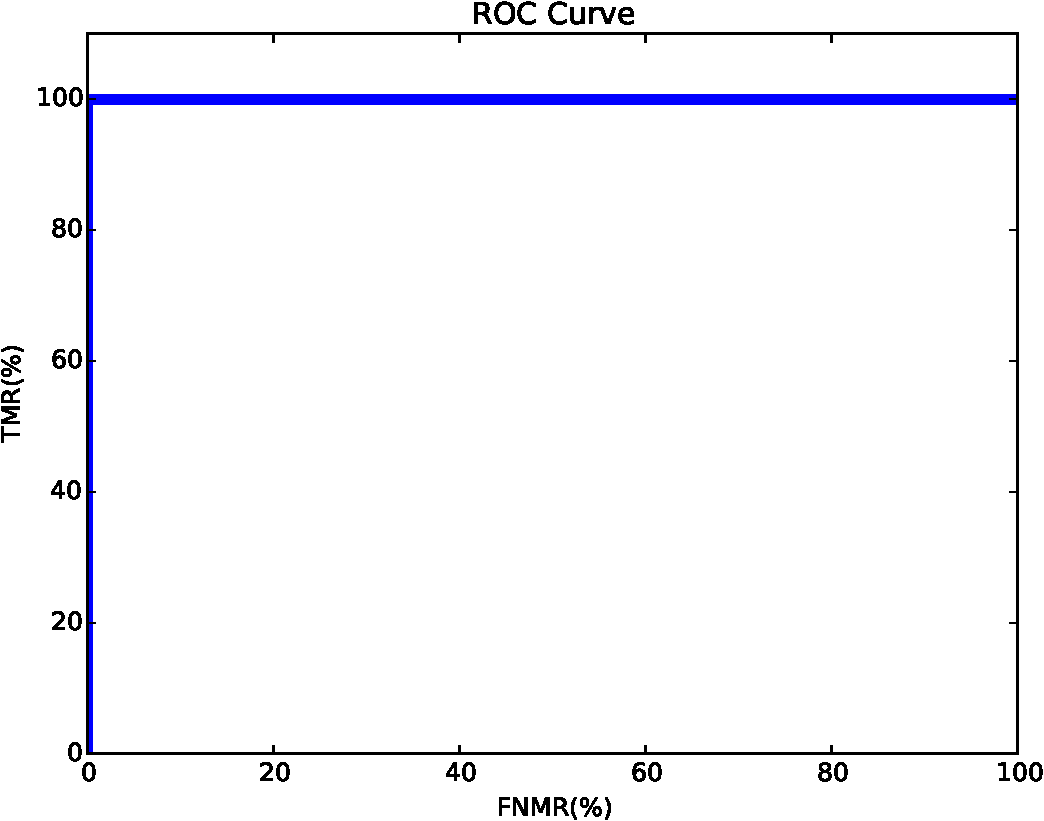
\includegraphics[scale=0.5]{fig-p12-crop}
\section*{Problem 3}
Yes, we can estimate recognition error rates from verification error rates.
First, view error rates as probilities.

Suppose there are $n$ people on the list.

For any person $P$ on the list. 
$$
\begin{aligned}
    &\Pr(\text{False Negative}) \\ 
    =&\Pr(P \text{ is not recognized as himself})\times\Pr(P \text{ is not recognized as other } n-1 \text{ people on the list})\\
    =&\text{FRR}\times(\text{TRR})^{n-1}=\text{FRR}\times(1-\text{FAR})^{n-1}
\end{aligned}
$$
For any person $P$ not on the list. 
$$
\begin{aligned}
    \Pr(\text{False Positive}) =&\Pr(P \text{ is recognized as someone on the list})\\
    =& 1 - \Pr(P \text{ is not recognized as anyone on the list})\\
    =& 1 - \text{TRR}^n = 1-(1-\text{FAR})^n
\end{aligned}
$$

Recognition is challenging, for the following reasons
\begin{itemize}
    \item To avoid mixing people up, we may need more accurate algorithms to verify each pairs of people in recognition problems.
    \item Since we have to compare one person with multiple persons every time in recognition, it is more difficult to make a recognition system efficient. 
\end{itemize}
\end{document}
